
%\graficarPDF{graf_ej3}{Estimación de la trayectoria.}{fig:ej3}

\begin{figure}[H]
\centering
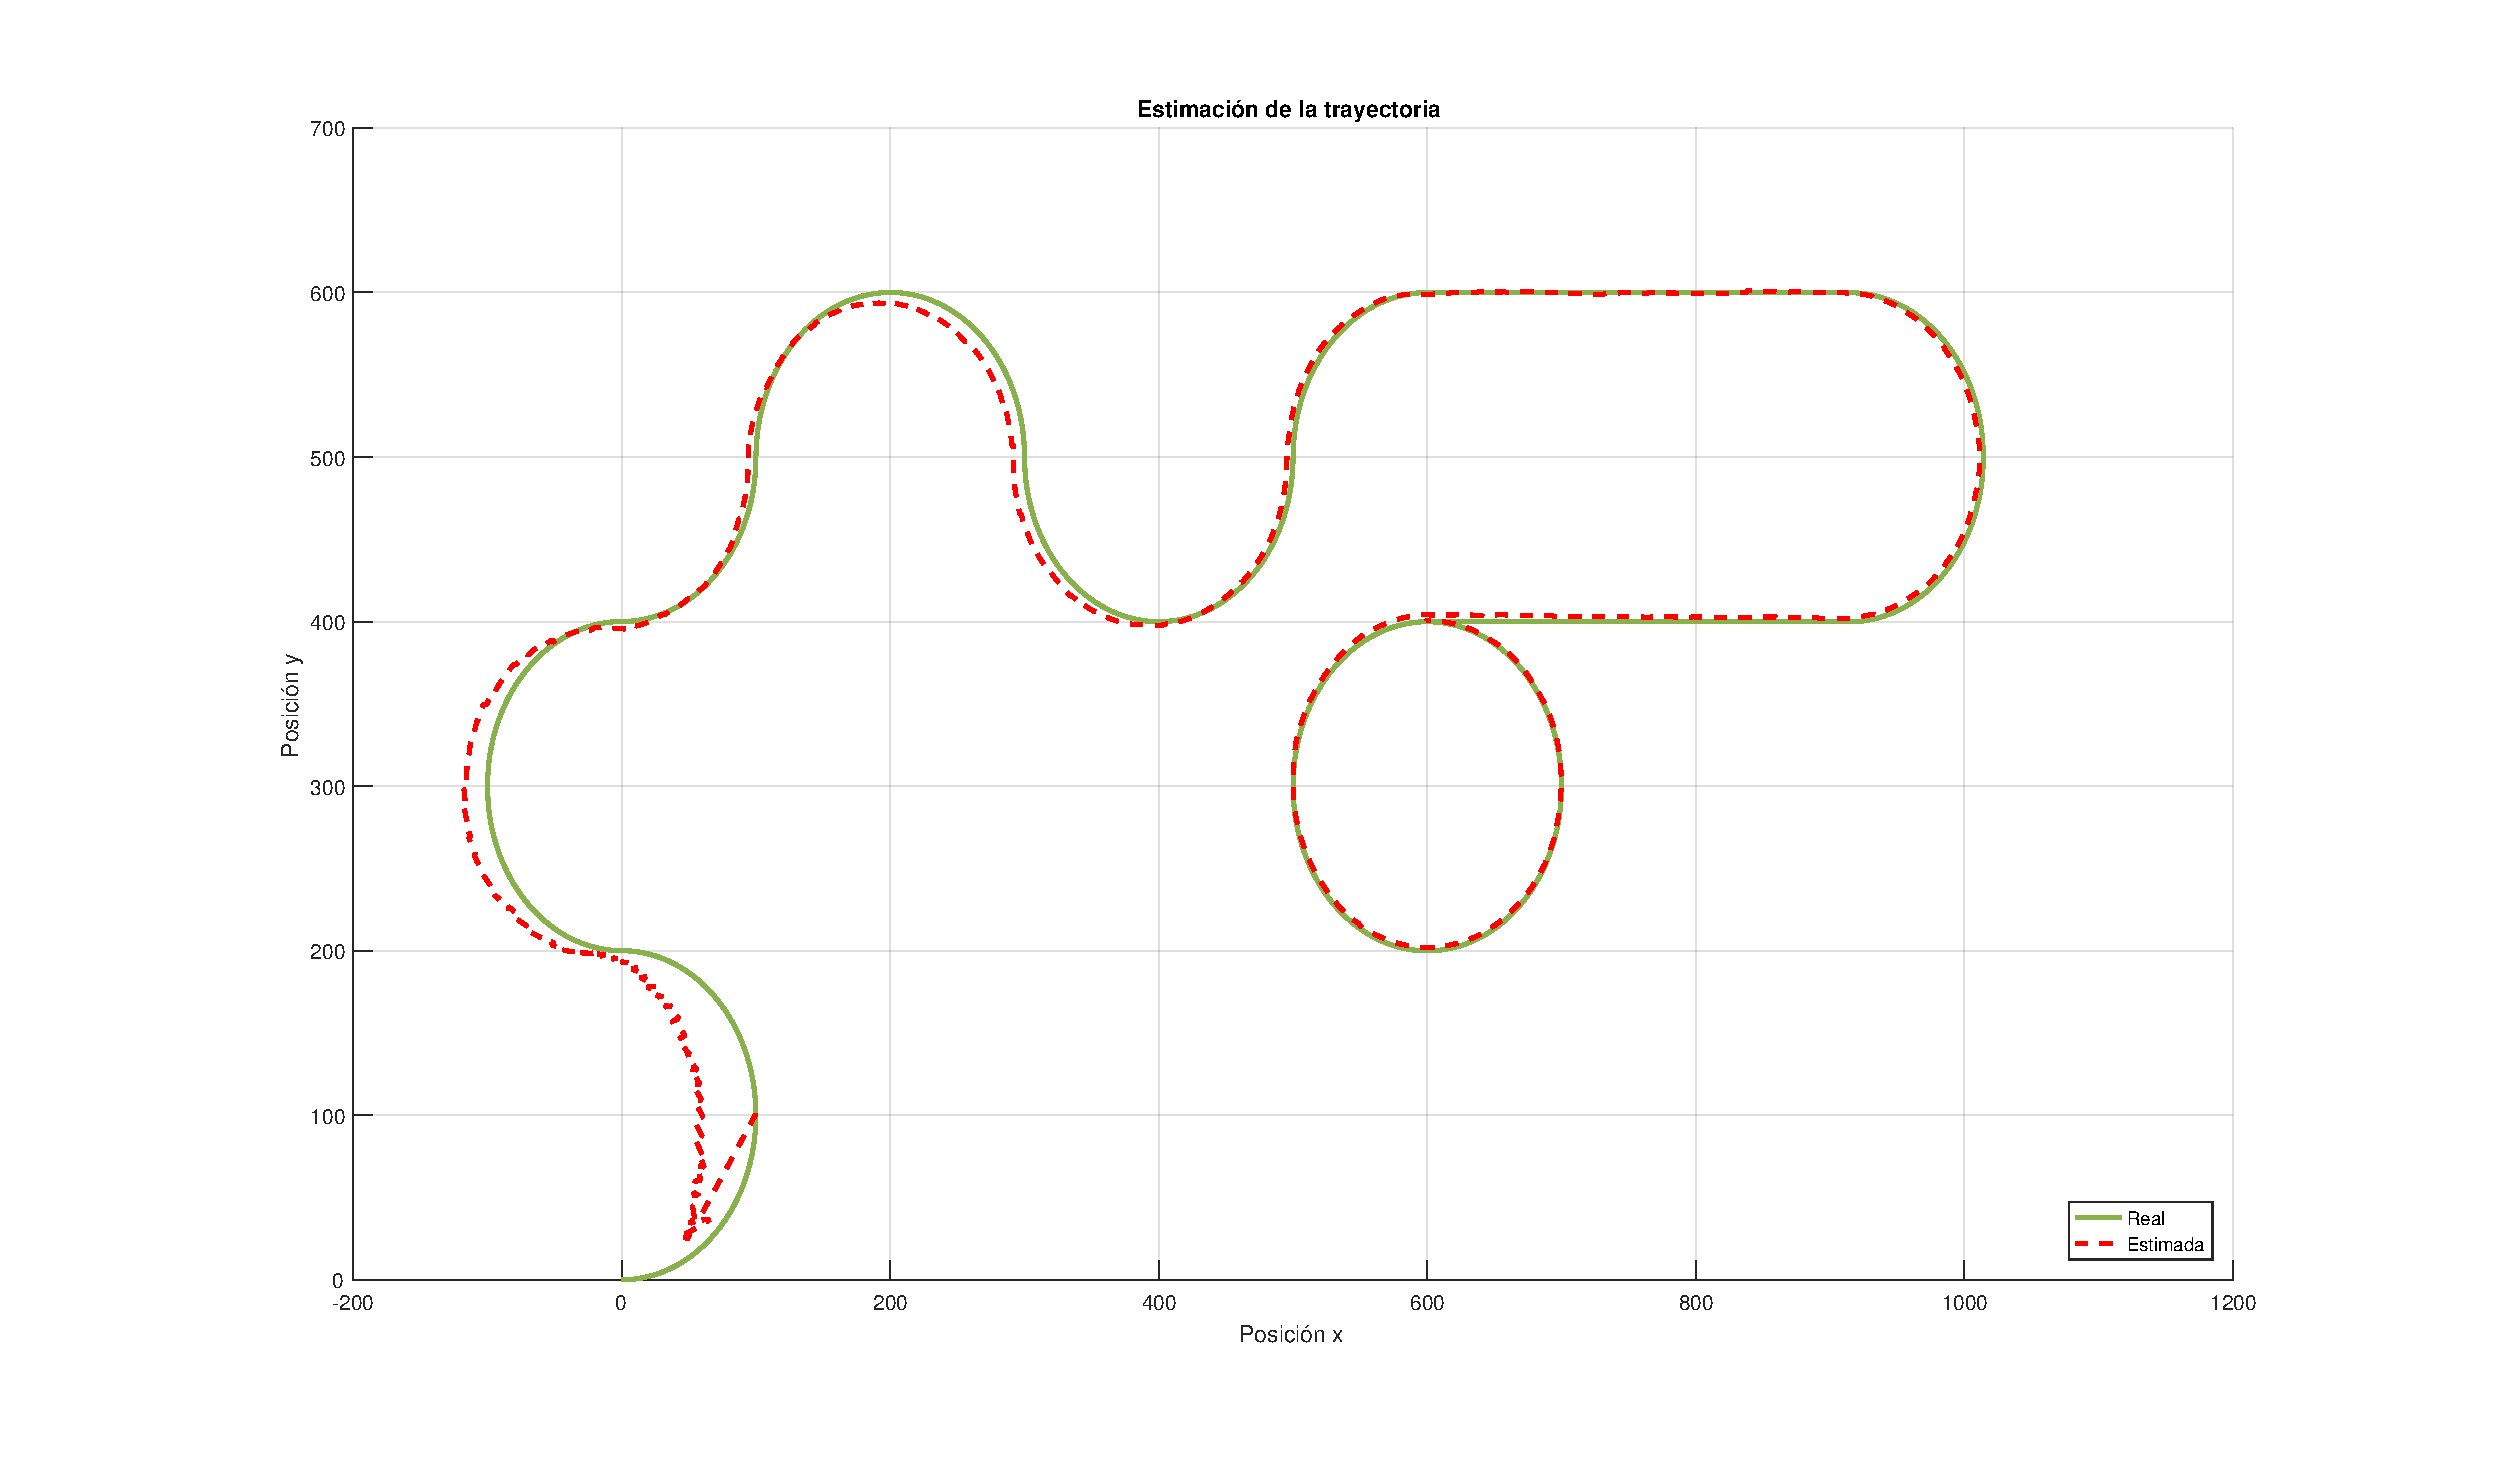
\includegraphics[width=\textwidth, trim= 2cm 2cm 2cm 2cm]{graf_ej3.pdf}
\caption{Estimación de la trayectoria.}
\label{fig:ej3} 
\end{figure}

	De la misma forma que en el trabajo previo, para la estimación del sesgo se lo agrega al vector de estados al sesgo en ambas coordenadas. Se supone que dicho sesgo es constante, por lo tanto la dinámica del mismo es constante y ruido de proceso nulo. Como el sesgo es en velocidad, a la matriz $C$ se le agregan 2 columnas cuyas dos últimas filas corresponden a la matriz identidad de $2\times 2$. Así las mediciones de velocidad tendrán adheridas los sesgos. Con lo expuesto, se obtiene la trayectoria de la Figura \ref{fig:ej3}. Realizando el test de observabilidad, se ve que todos los estados son observables. Viendo también las innovaciones en la Figura \ref{fig:3covinn} se confirma que las correlaciones son similares al de un proceso blanco asegurando que la estimación es correcta.\\ 

%\graficarPDF{graf_ej3_covinn}{Innovaciones de las posiciones y velocidades en $x^e$ e $y^e$.}{fig:3covinn}

\begin{figure}[H]
\centering
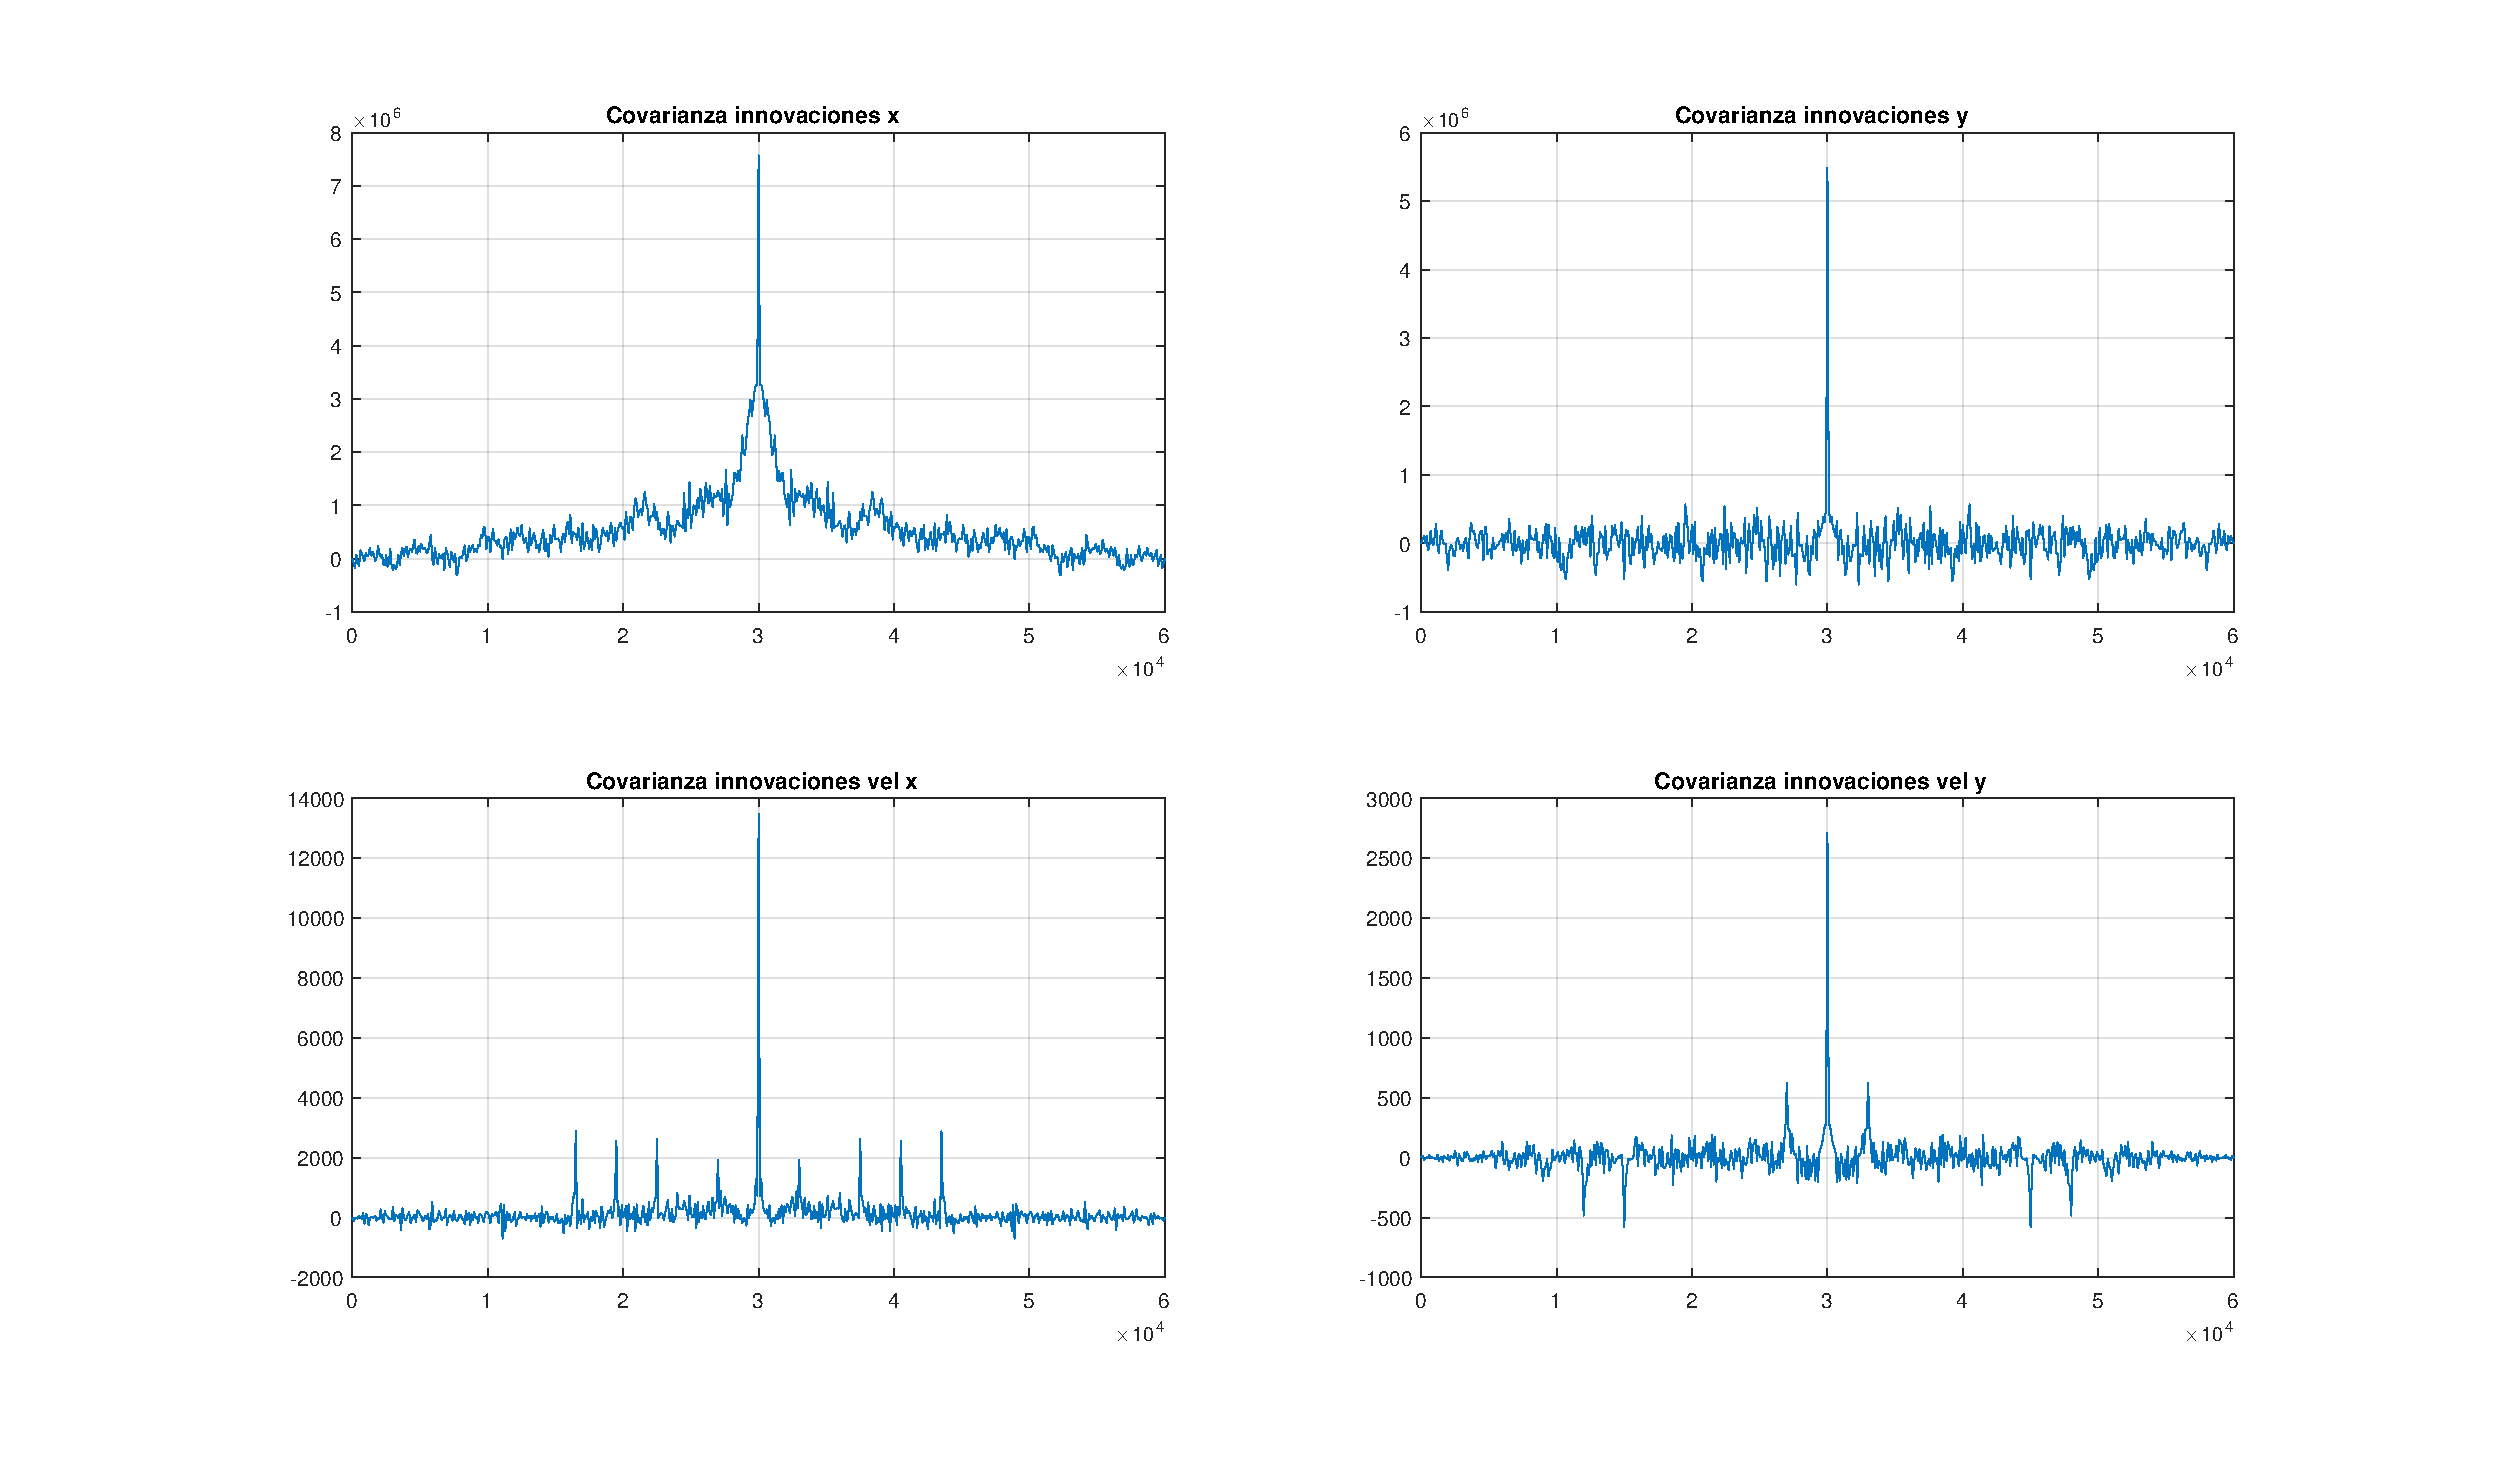
\includegraphics[width=0.9\textwidth,trim= 2cm 2cm 2cm 2cm]{graf_ej3_covinn.pdf}
\caption{Innovaciones de las posiciones y velocidades en $x^e$ e $y^e$.}
\label{fig:3covinn} 
\end{figure}

\pagebreak


%\graficarPDFa{0 05cm 0 13cm}{graf_ej3_pos}{Posición y error de la misma en función del tiempo.}{fig:3pos}

\vspace*{\fill}
\begin{figure}[H]
\centering
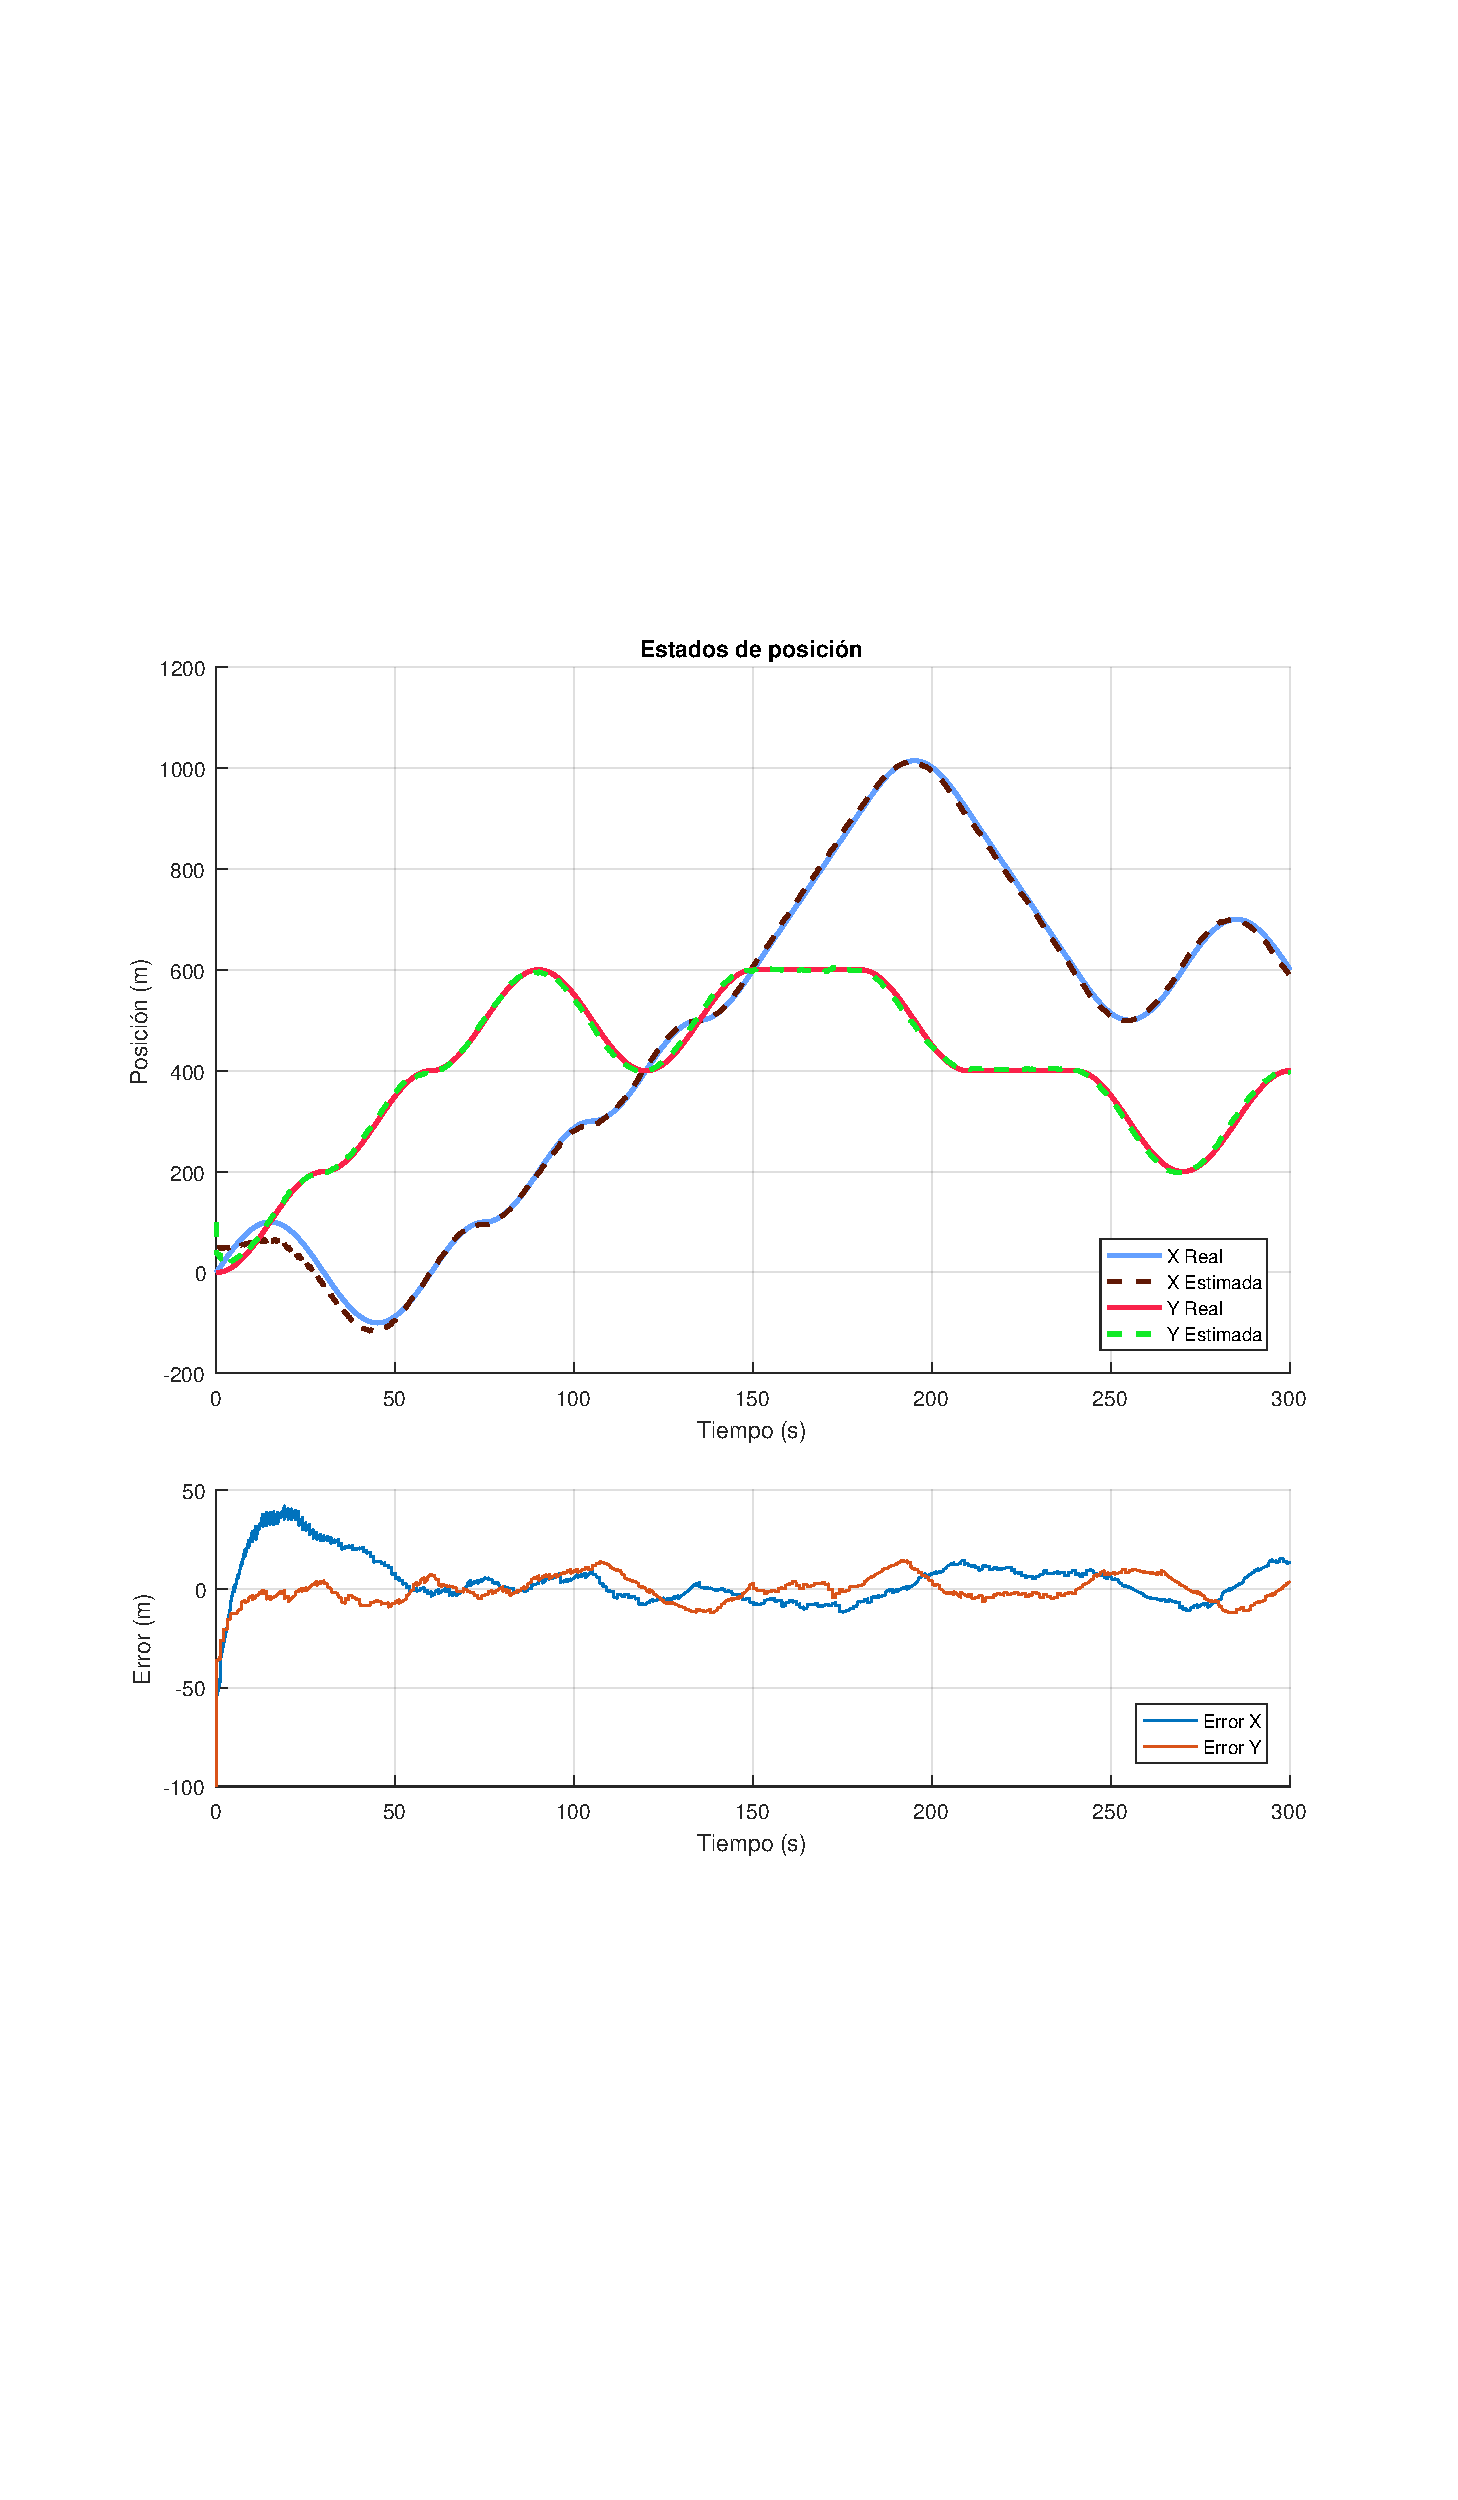
\includegraphics[scale=0.5, trim= 6cm 6cm 6cm 6cm]{graf_ej3_pos.pdf}
\caption{Posición y error de la misma en función del tiempo.}
\label{fig:3pos} 
\end{figure}
\vspace*{\fill}

\pagebreak


%\graficarPDFa{0 05cm 0 15cm}{graf_ej3_vel}{Velocidad real y estimada en función del tiempo.}{fig:3vel}

\vspace*{\fill}
\begin{figure}[H]
\centering
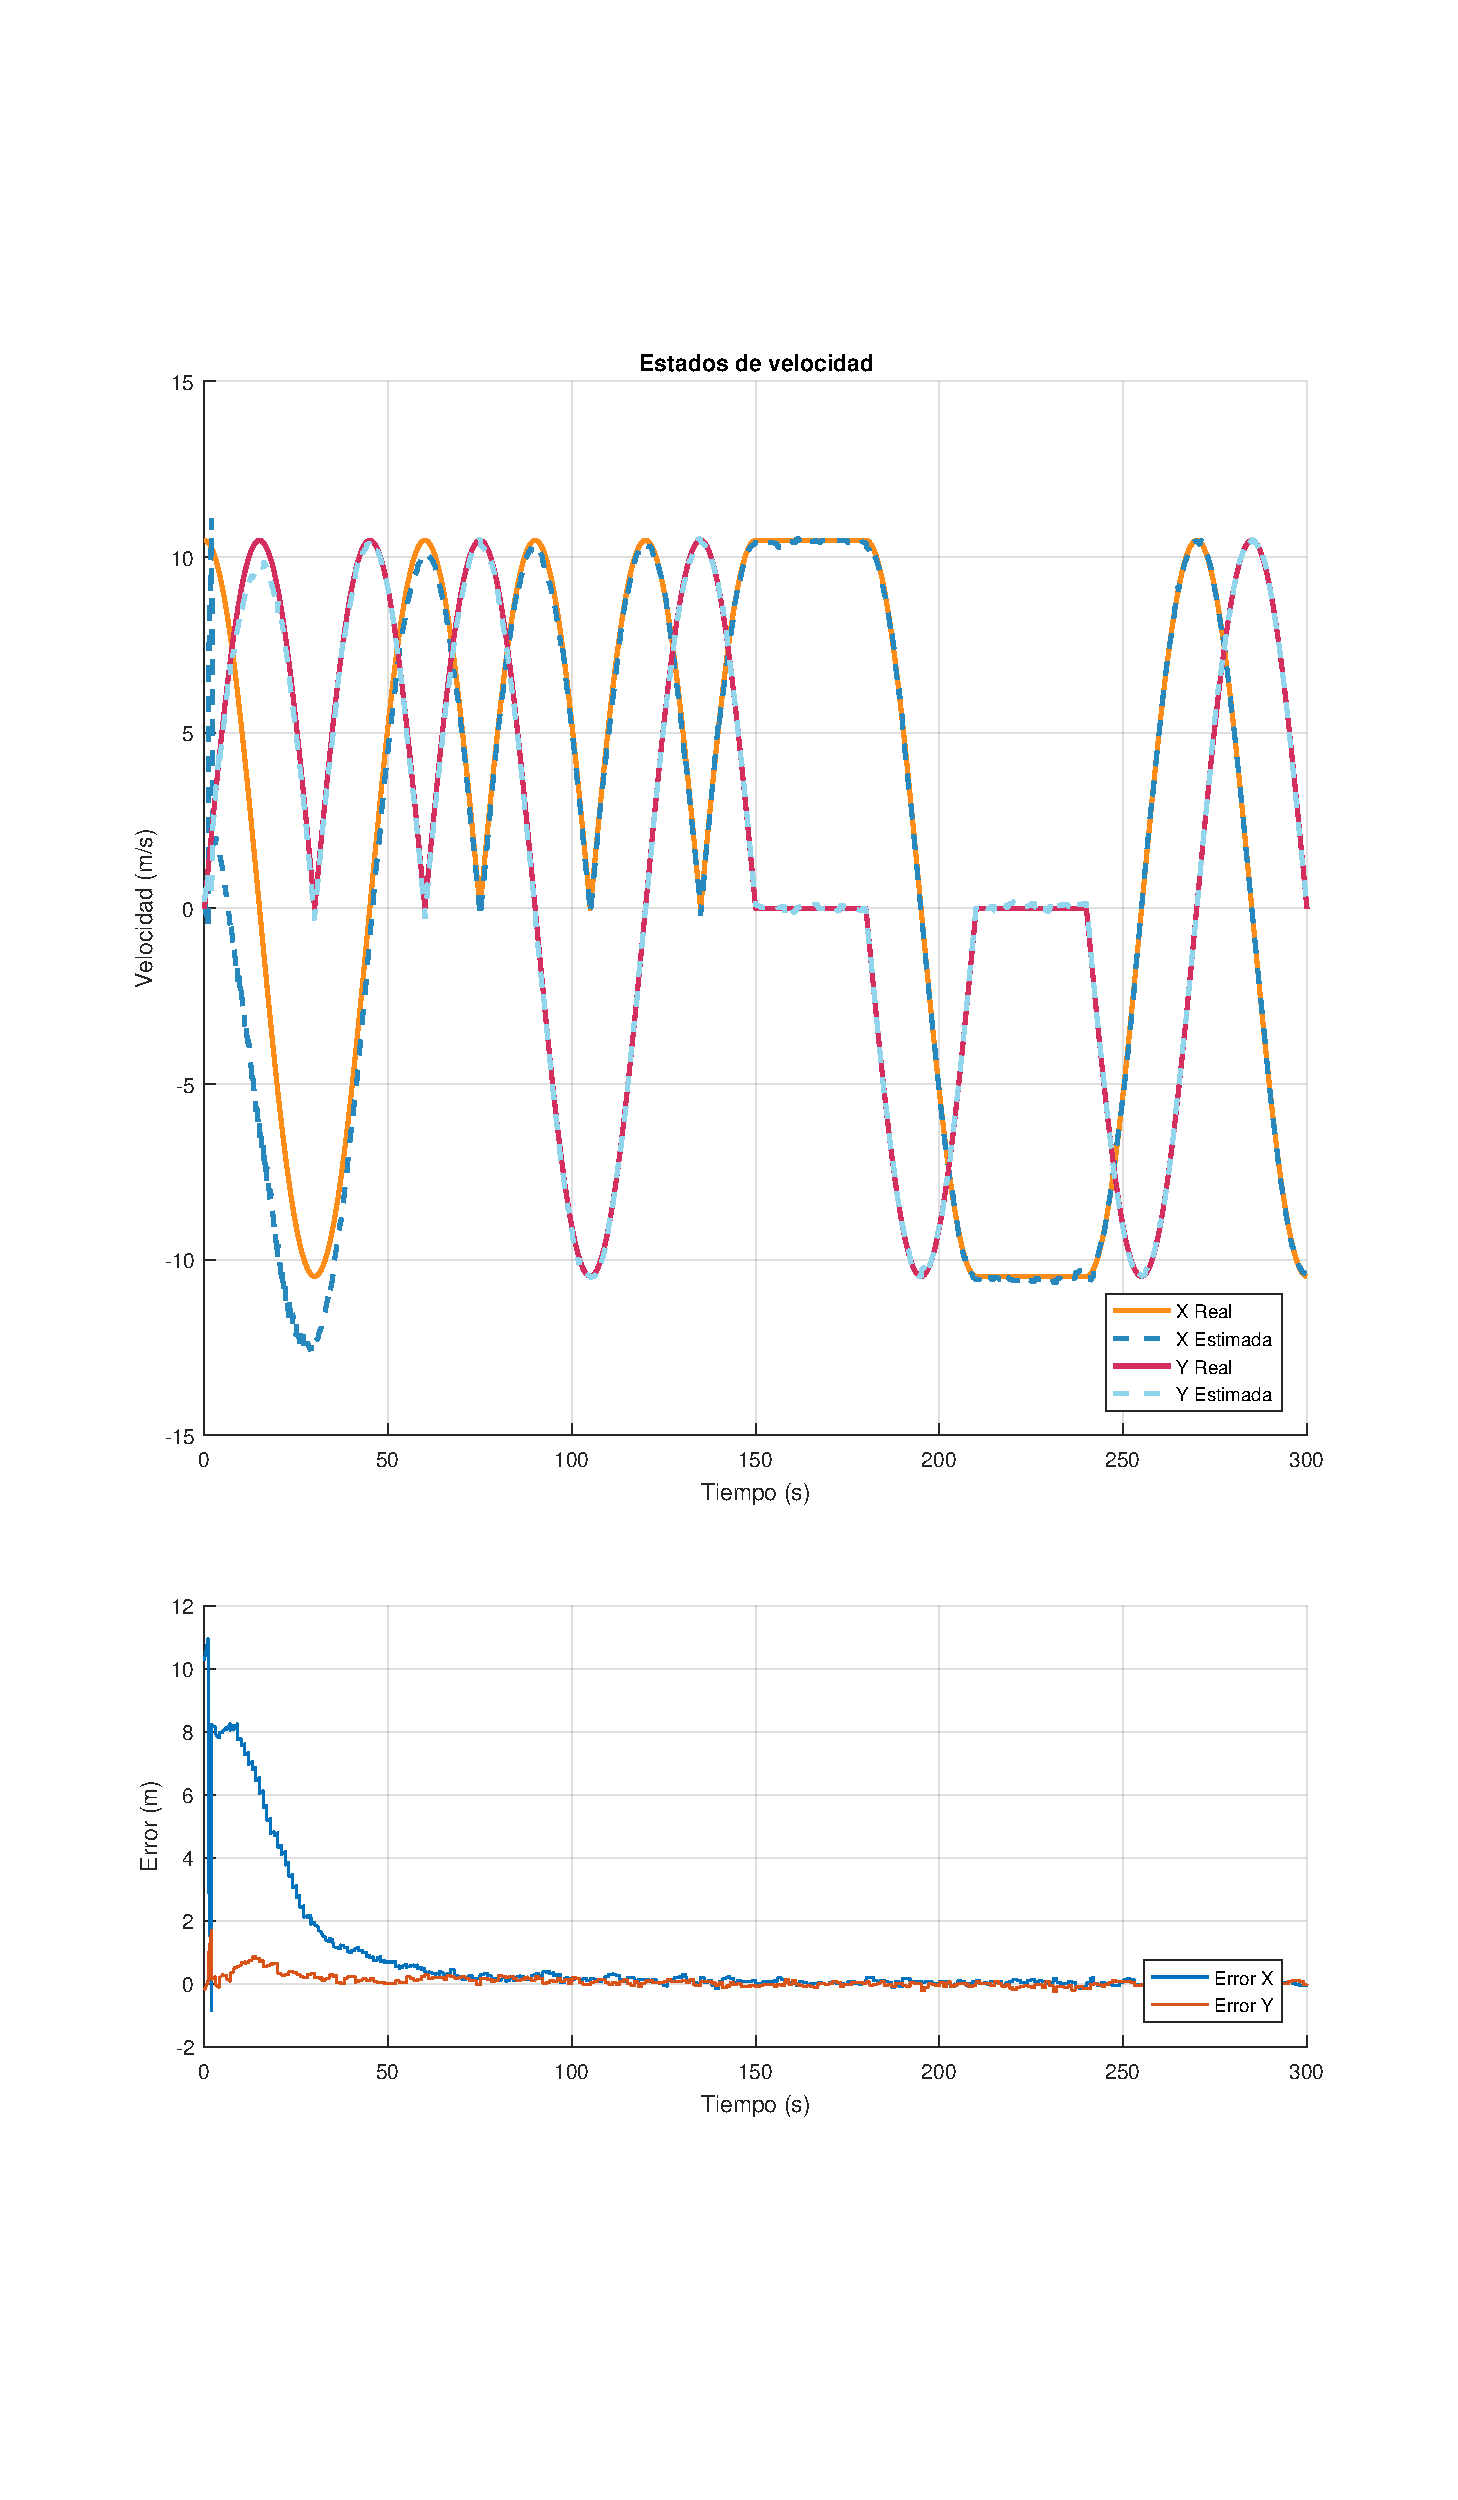
\includegraphics[scale=0.5, trim= 5cm 5cm 5cm 5cm]{graf_ej3_vel.pdf}
\caption{Velocidad real y estimada en función del tiempo.}
\label{fig:3vel} 
\end{figure}
\vspace*{\fill}

\pagebreak

\vspace*{\fill}
\graficarPDF{graf_ej3_theta}{Valores de los coeficientes de $C^e_b$ en el tiempo.}{fig:3theta}
\vspace*{\fill}